\section{DD}

	\begin{frame}[plain]
		\vfill
		\centering
		\begin{beamercolorbox}[sep=8pt,center,shadow=true,rounded=true]{title}
			\textbf{\usebeamerfont{title}\insertsectionhead}\par%
			\color{polimiblue}\noindent\rule{10cm}{1pt} \\
		\end{beamercolorbox}
		\vfill
	\end{frame}

	\subsection{Component View}
		\begin{frame}{High-Level View}
			\centering
			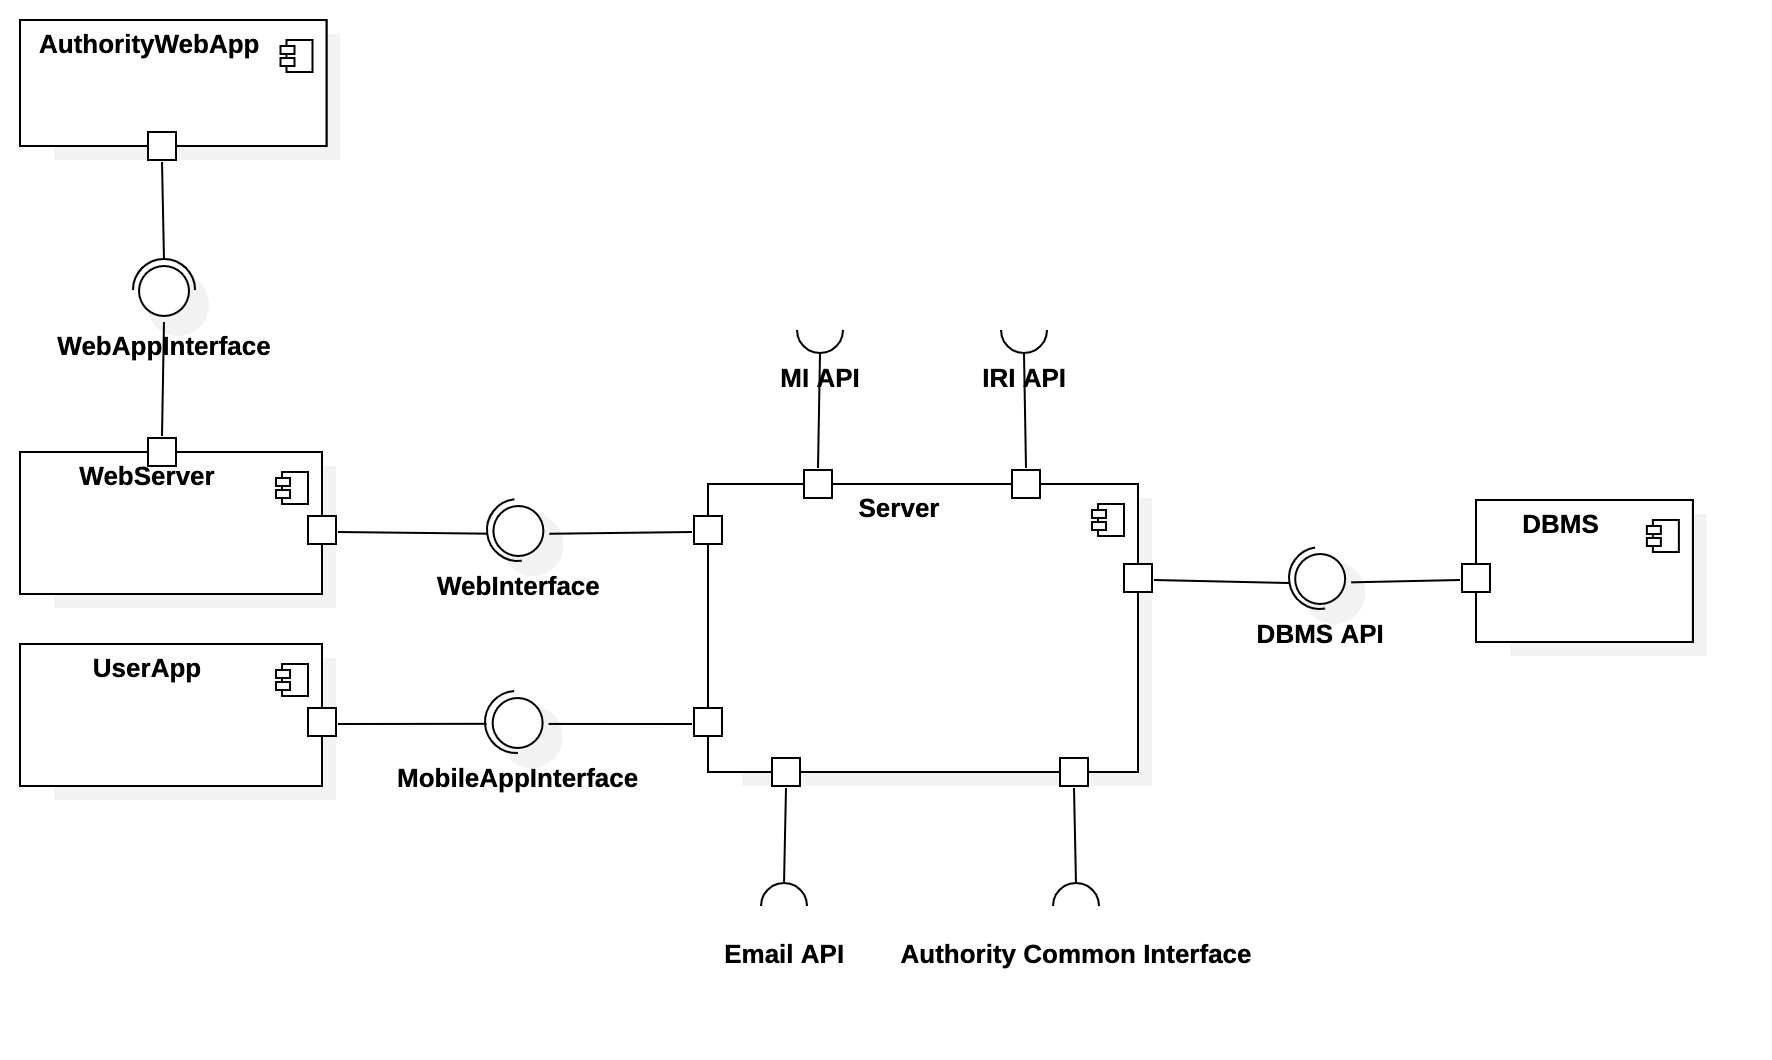
\includegraphics[scale=0.18]{dd/highLevel}
		\end{frame}
	
		\begin{frame}{Server Component}
			\noindent\makebox[\textwidth]{%
			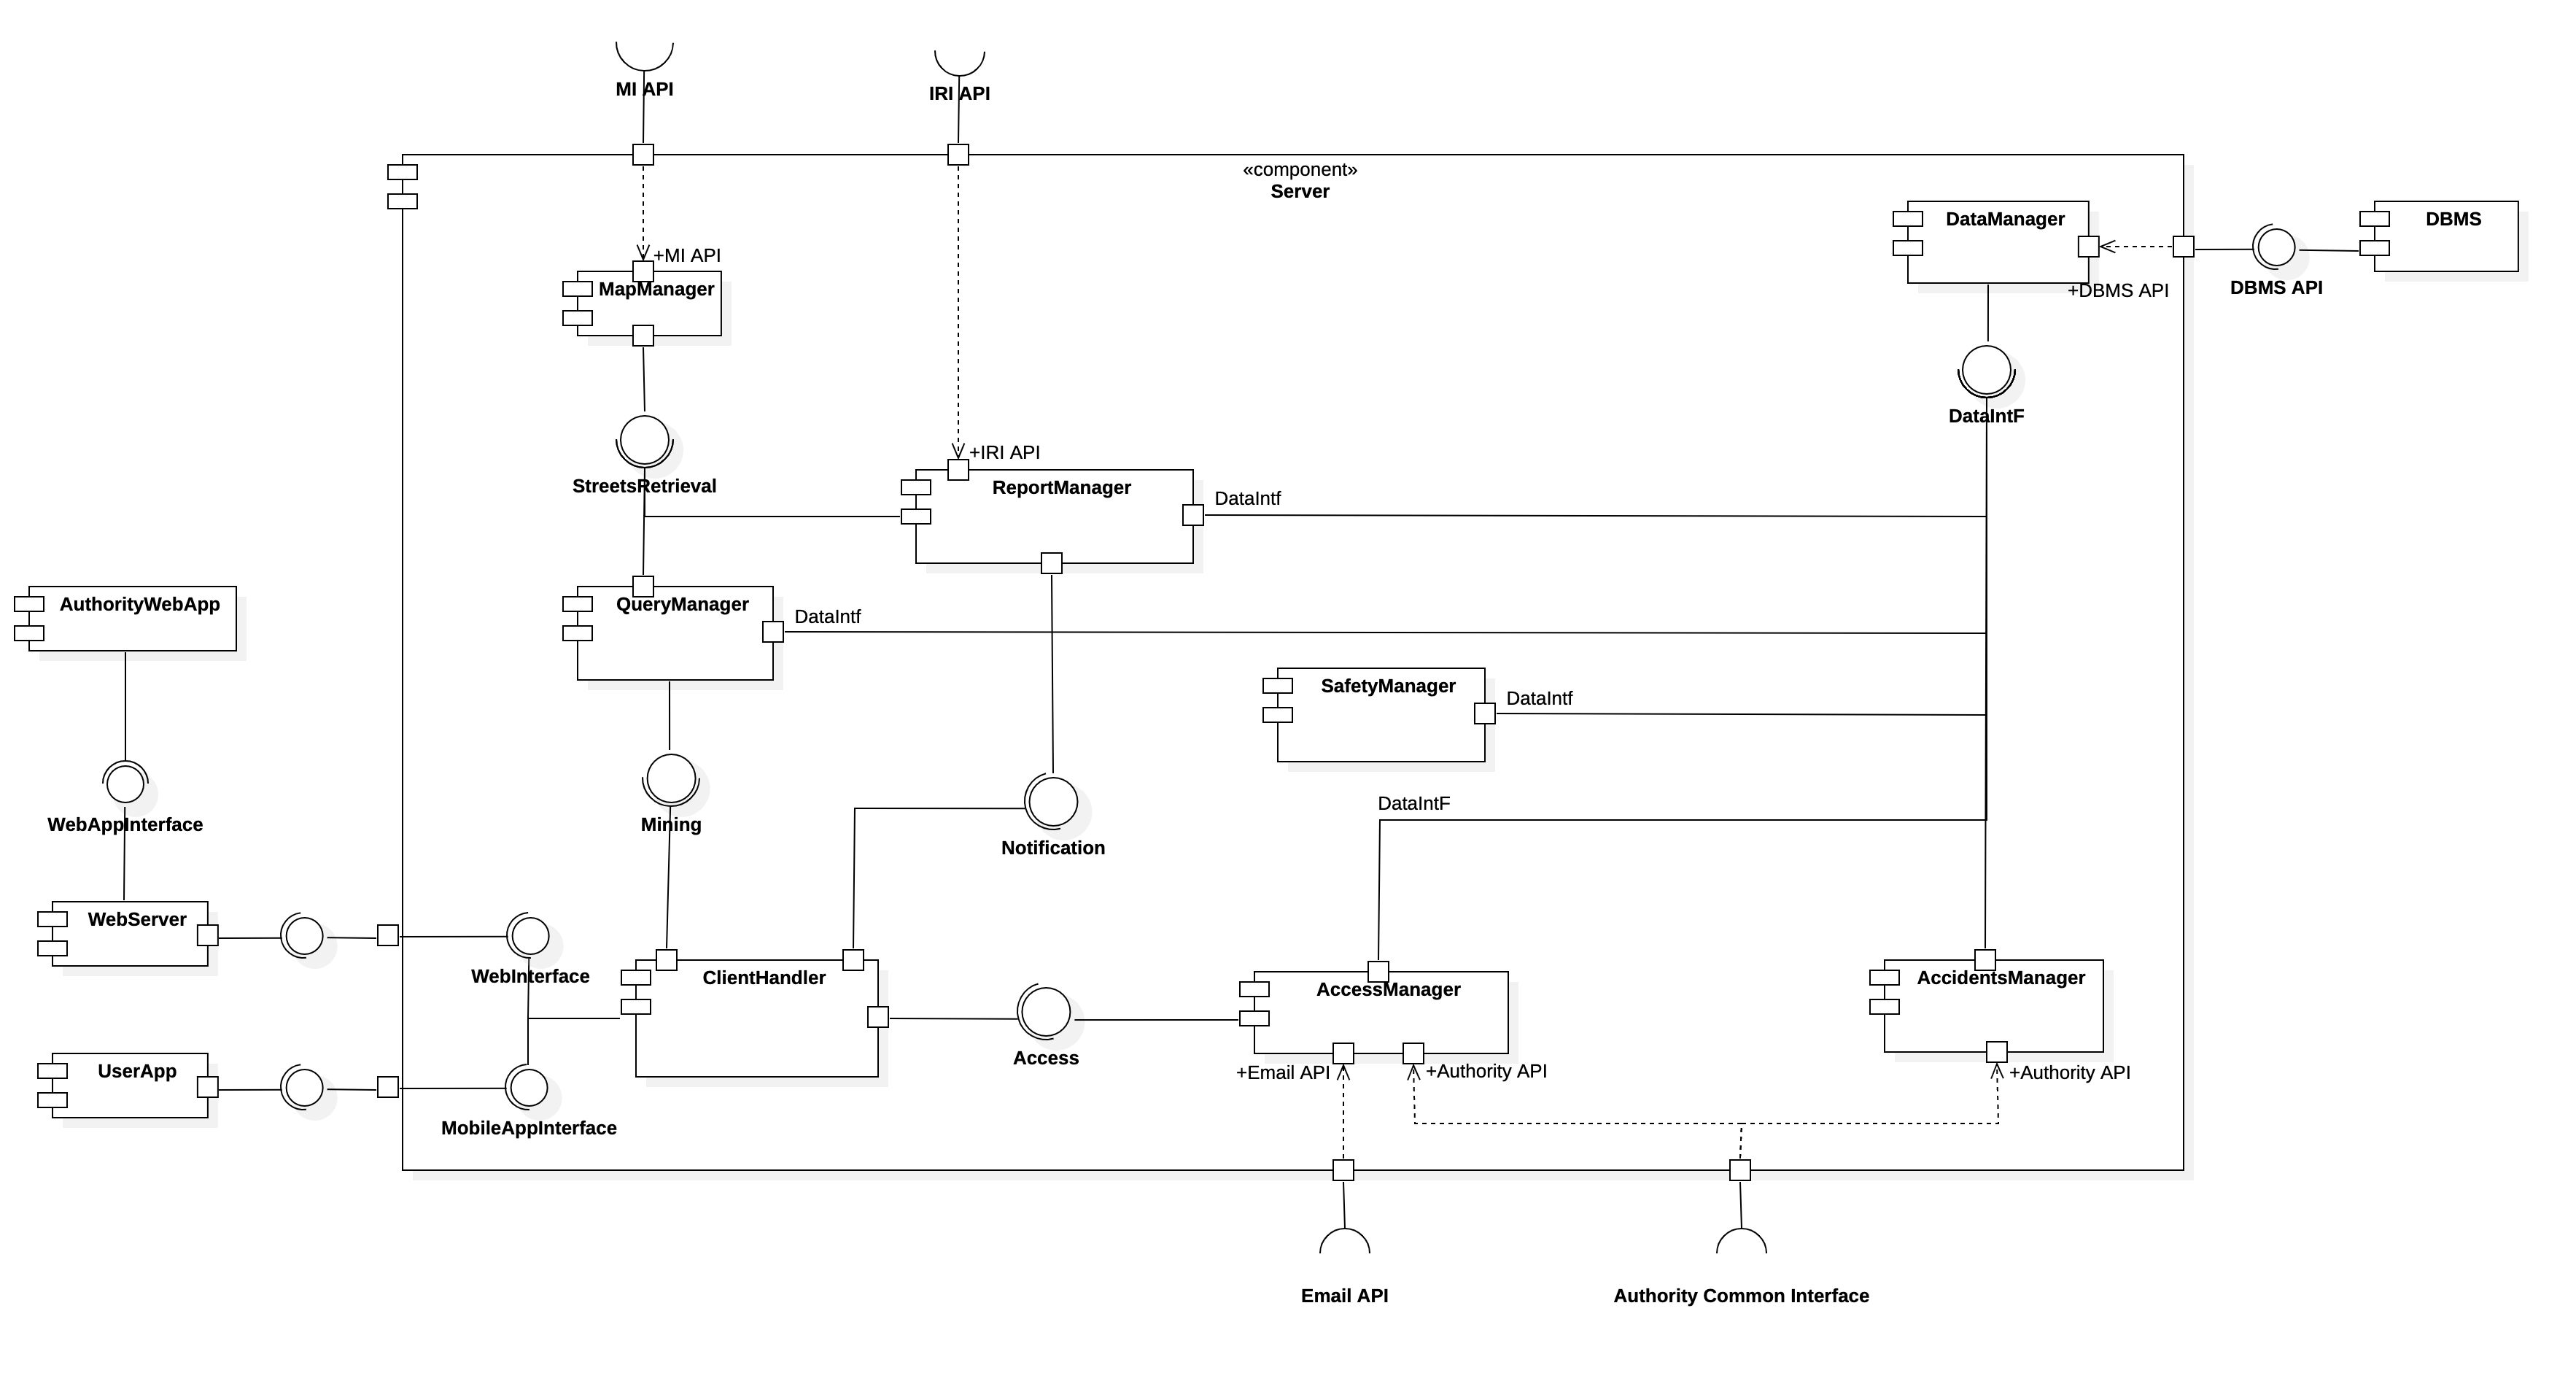
\includegraphics[width=1.2\textwidth]{dd/server}}
		\end{frame}
	
	\subsection{Components Interfaces}
		\begin{frame}{Component Interfaces}
			\vspace{-6pt}
			\noindent\makebox[\textwidth]{%
			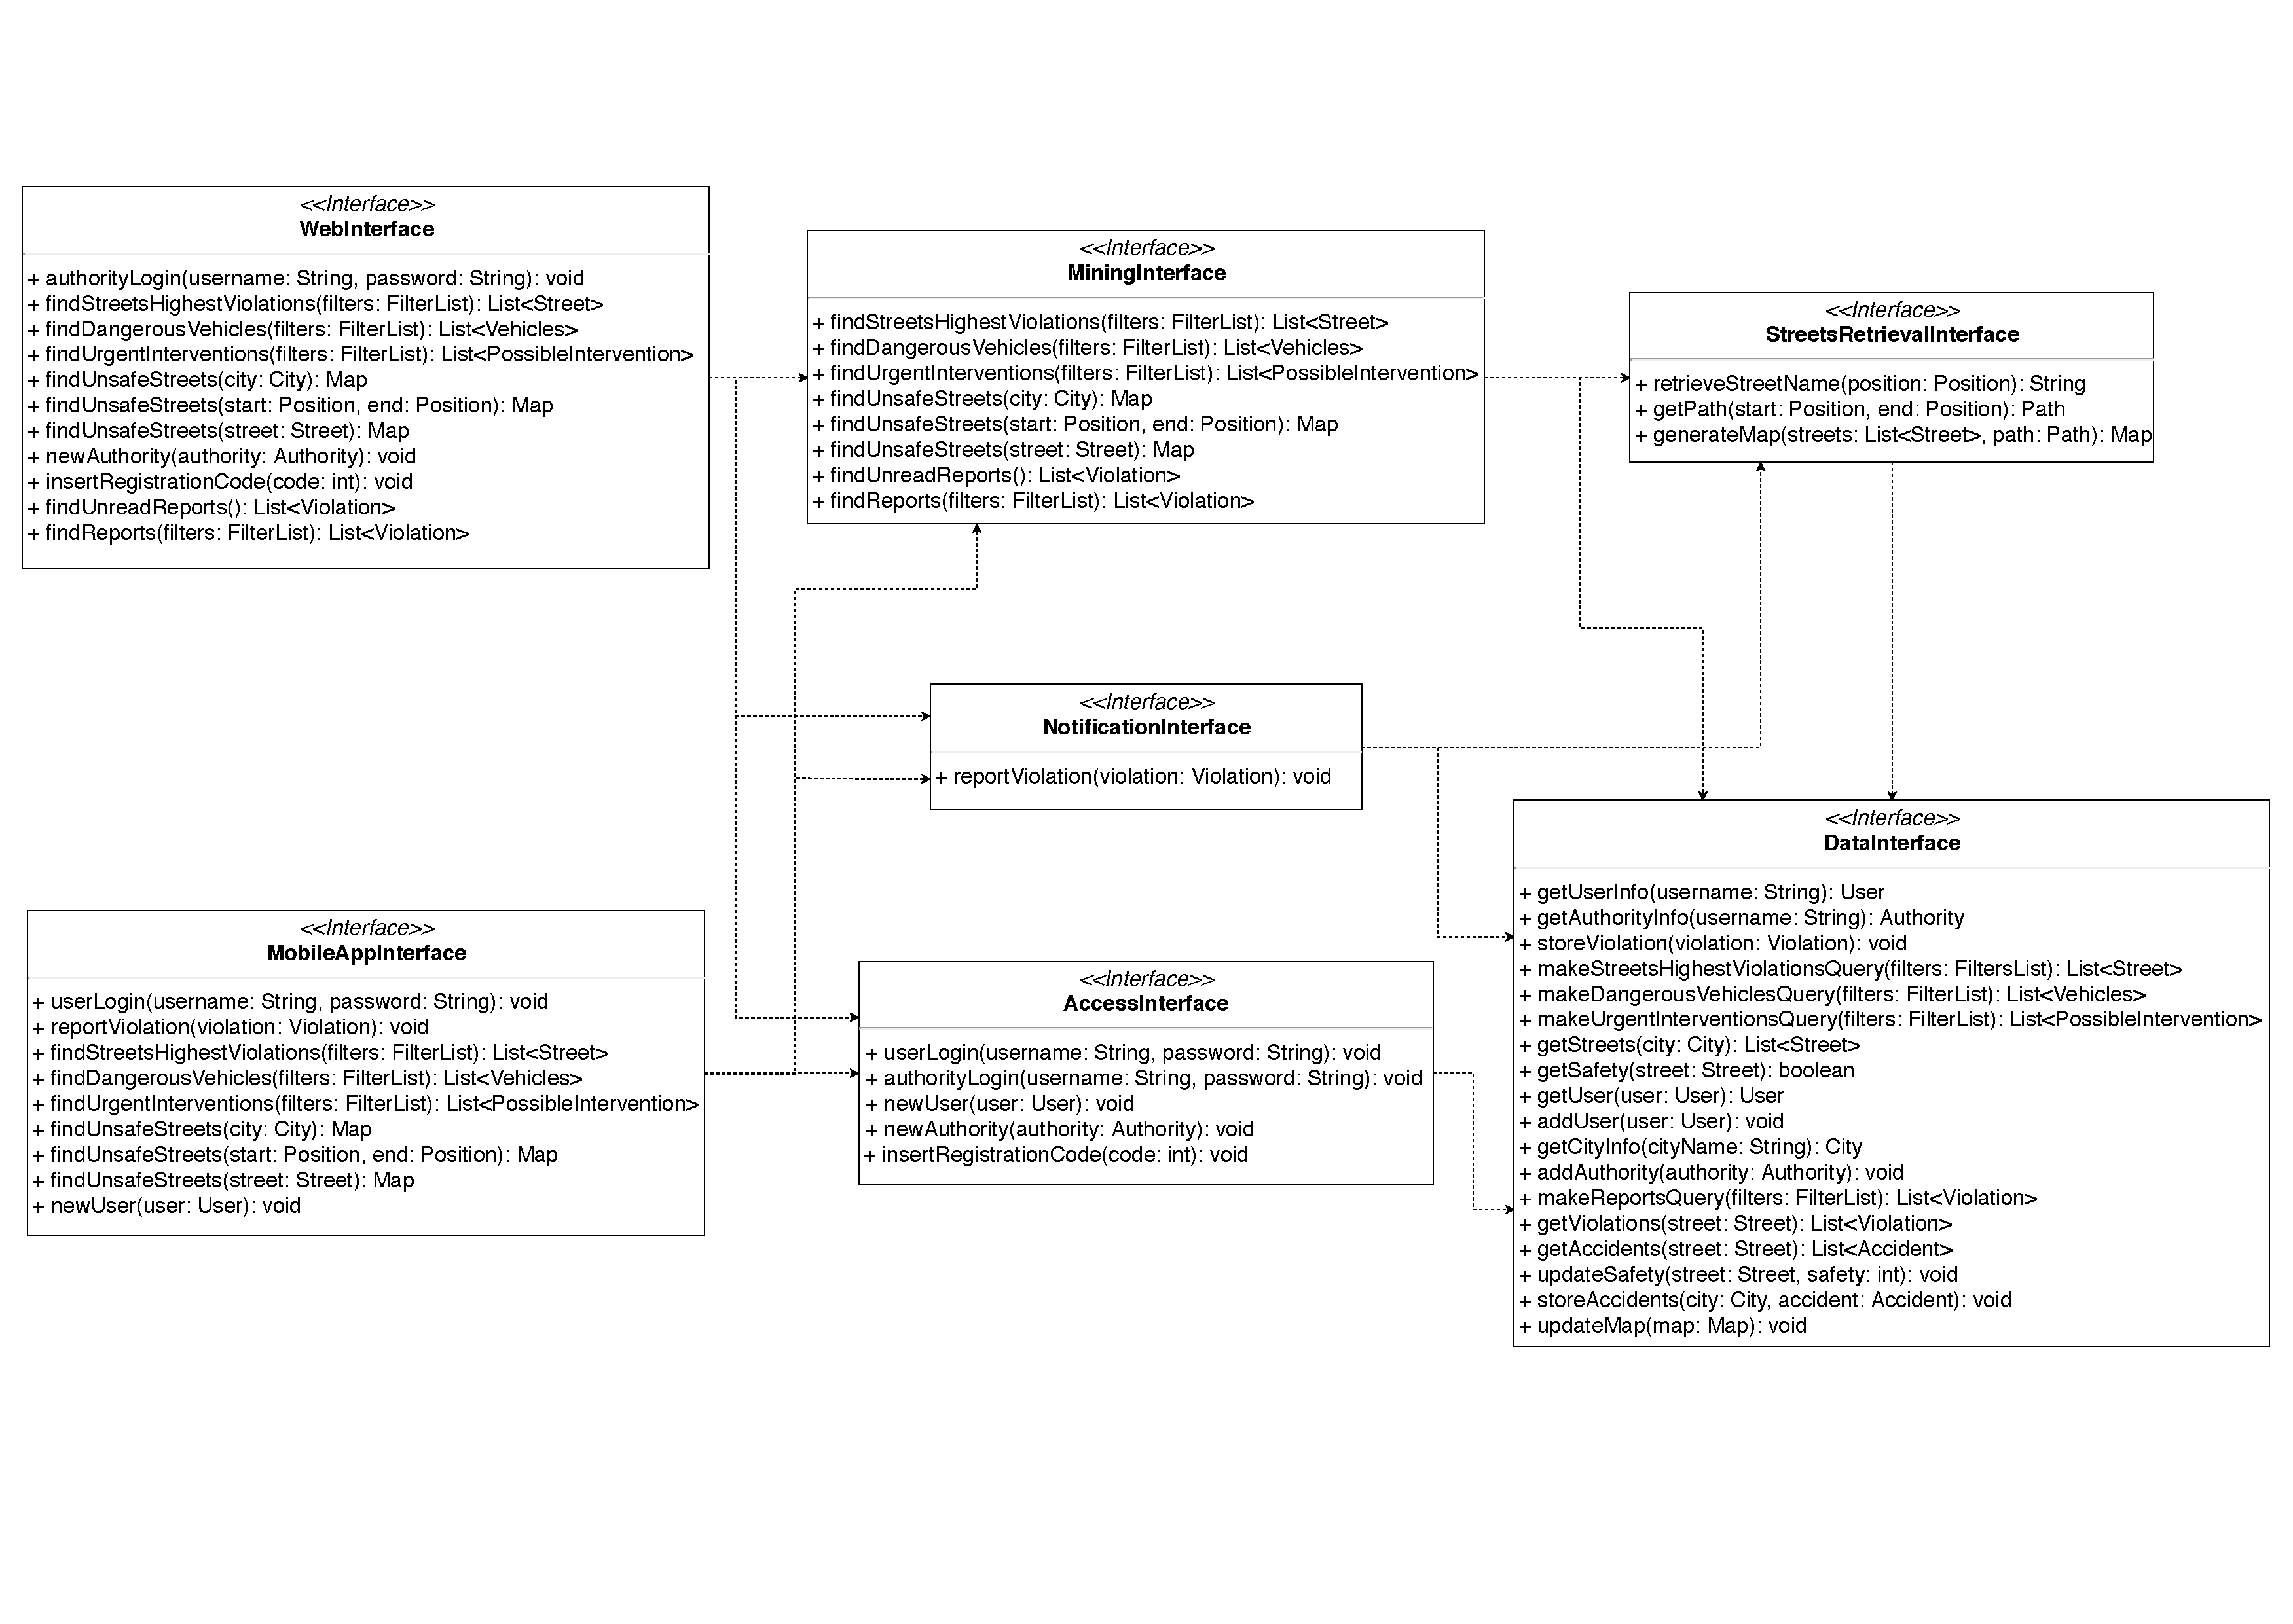
\includegraphics[scale=0.21]{dd/componentInterfaces}}
		\end{frame}
	
	\subsection{Runtime View}
		\begin{frame}{Report Violation and Find Reports}
			\vspace{-5pt}
			\begin{figure}
				\centering
				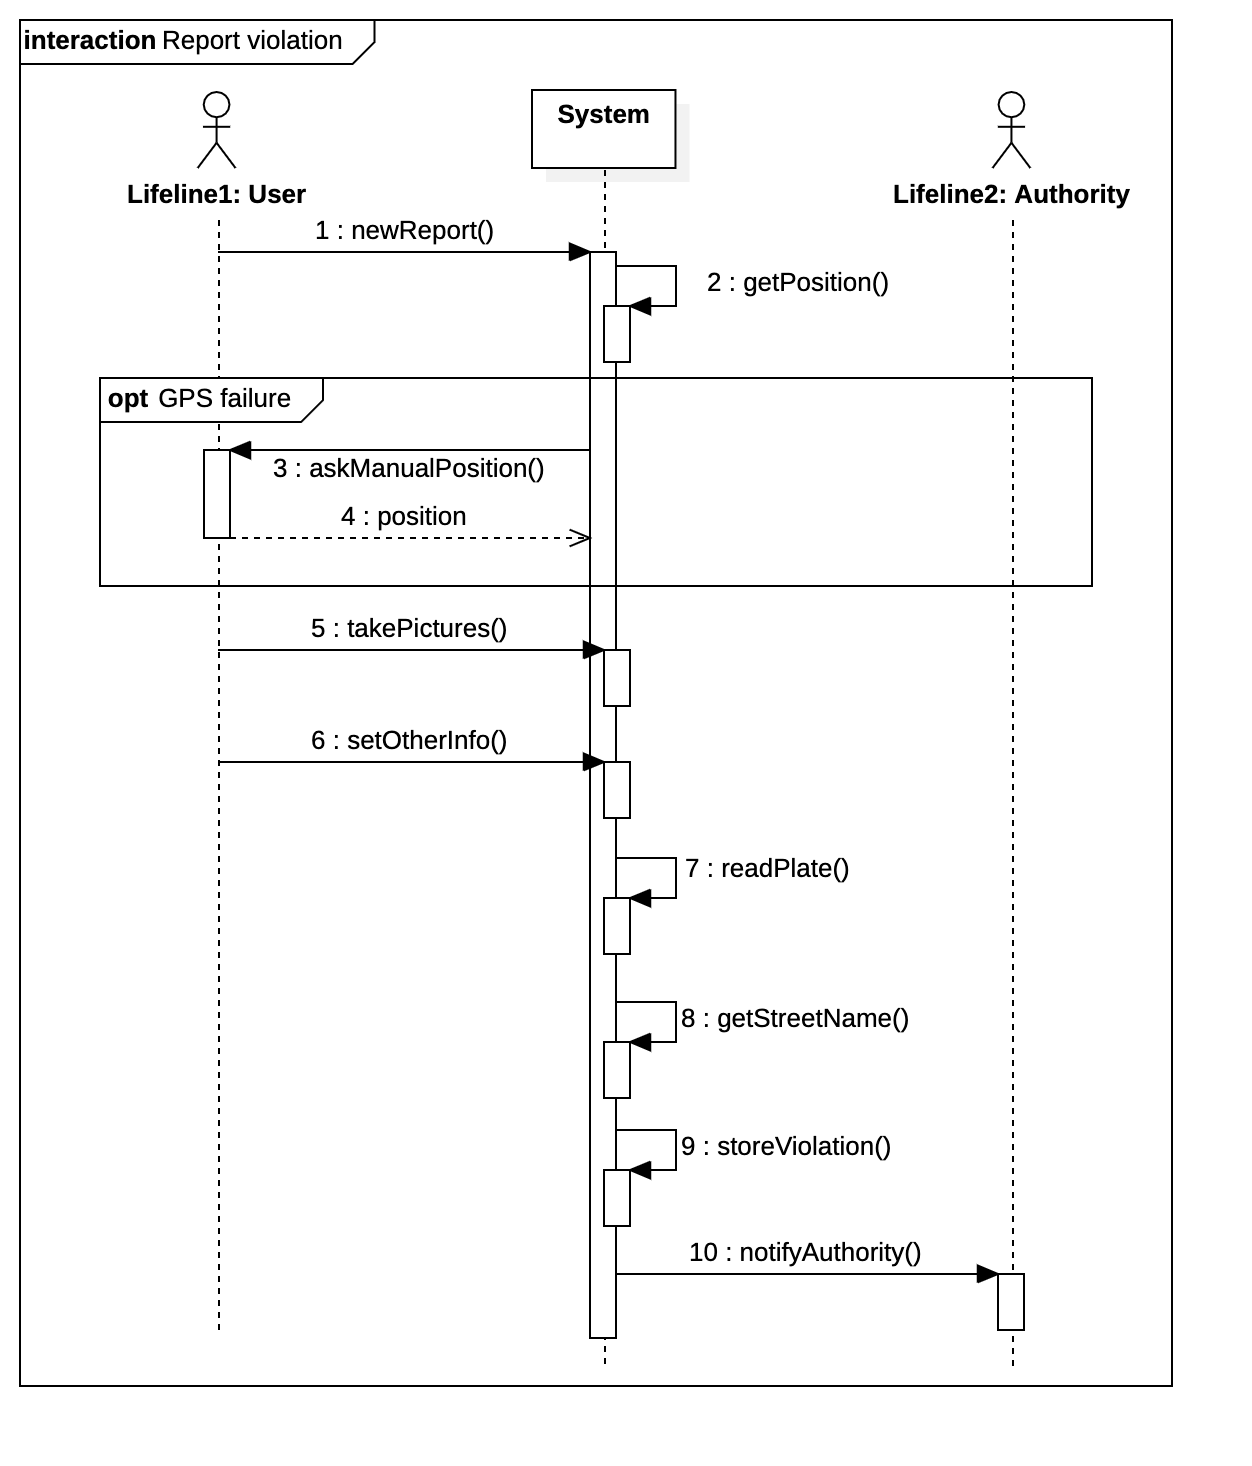
\includegraphics[scale=0.12]{dd/reportViolation}
			\end{figure}
			\vspace{-10pt}
			\begin{figure}
				\centering
				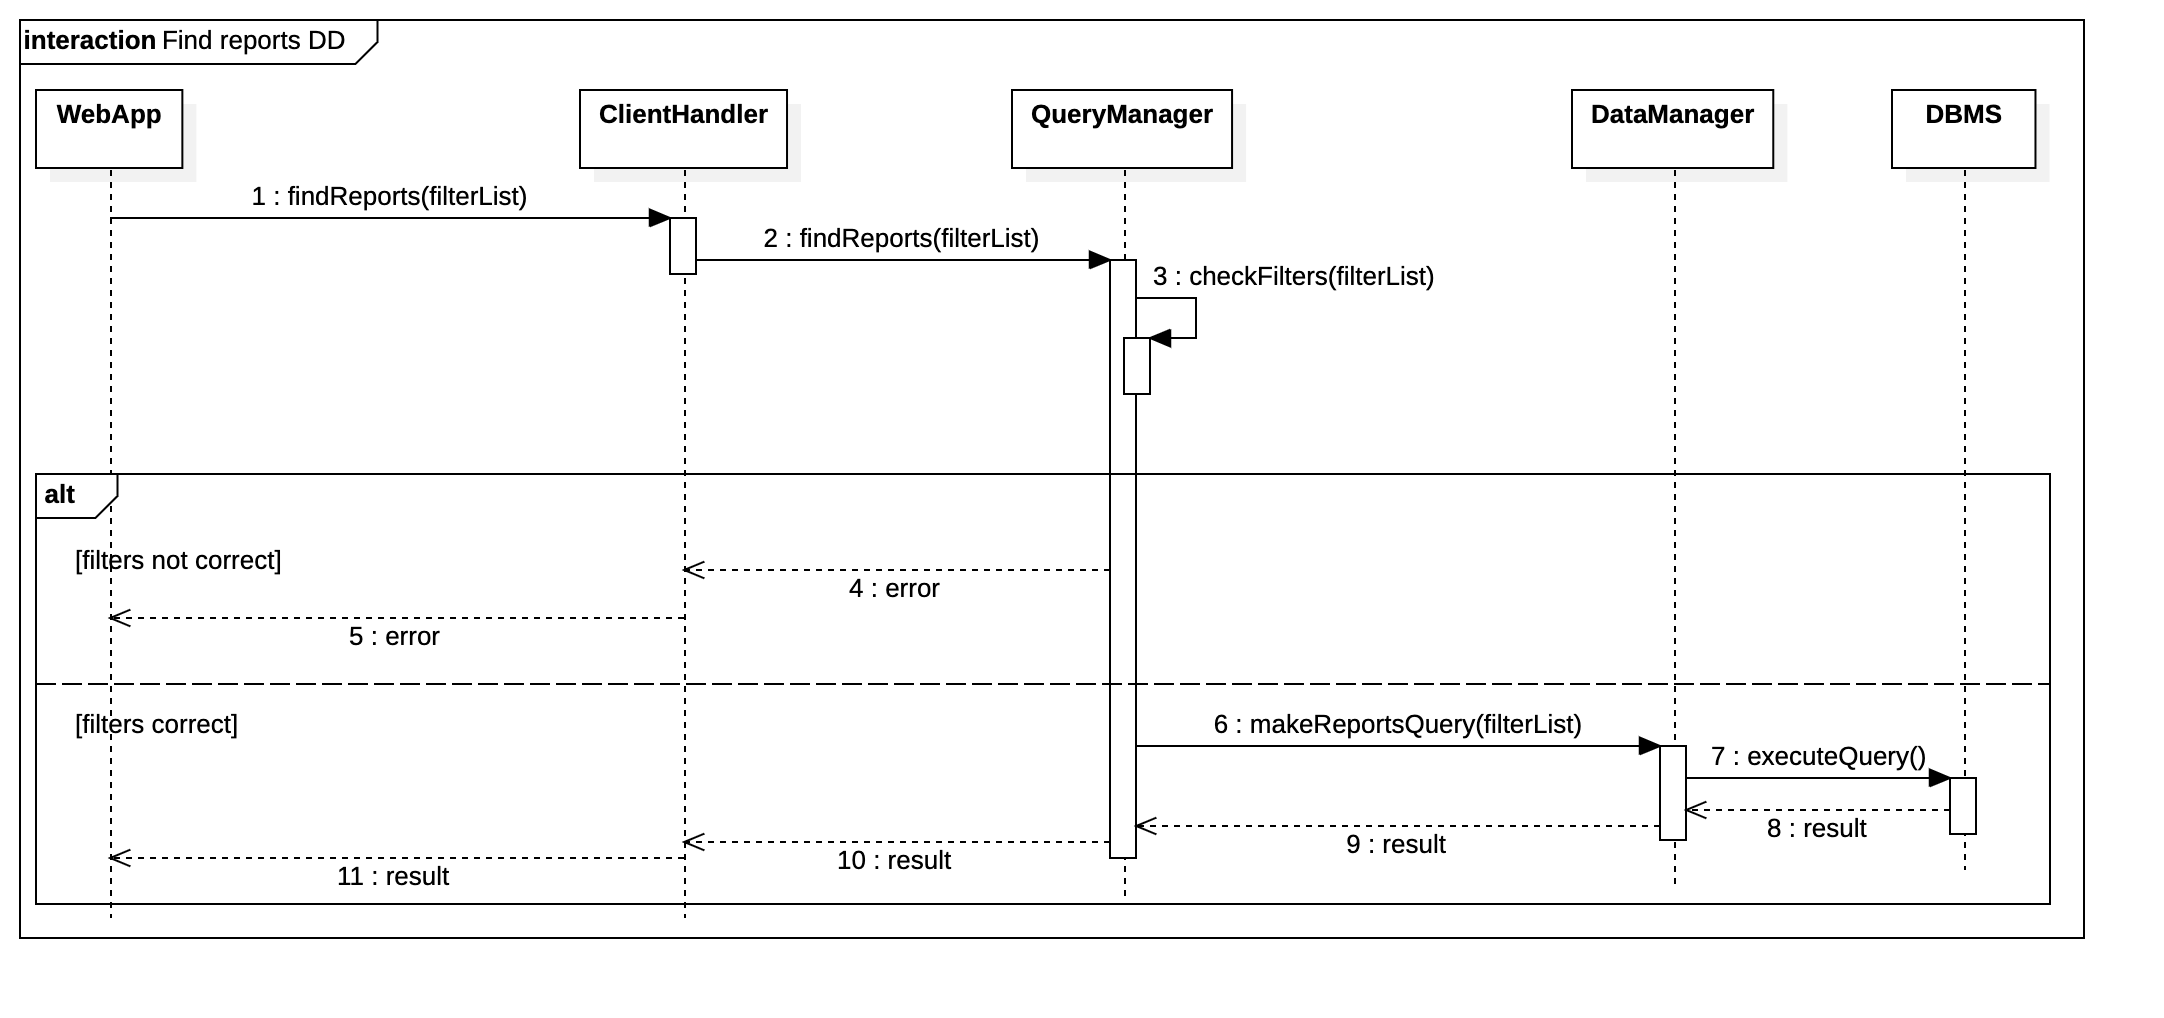
\includegraphics[scale=0.12]{dd/findReports}
			\end{figure}
		\end{frame}
	
		\begin{frame}{Update Safety}
			\begin{figure}[hbtp]
				\centering
				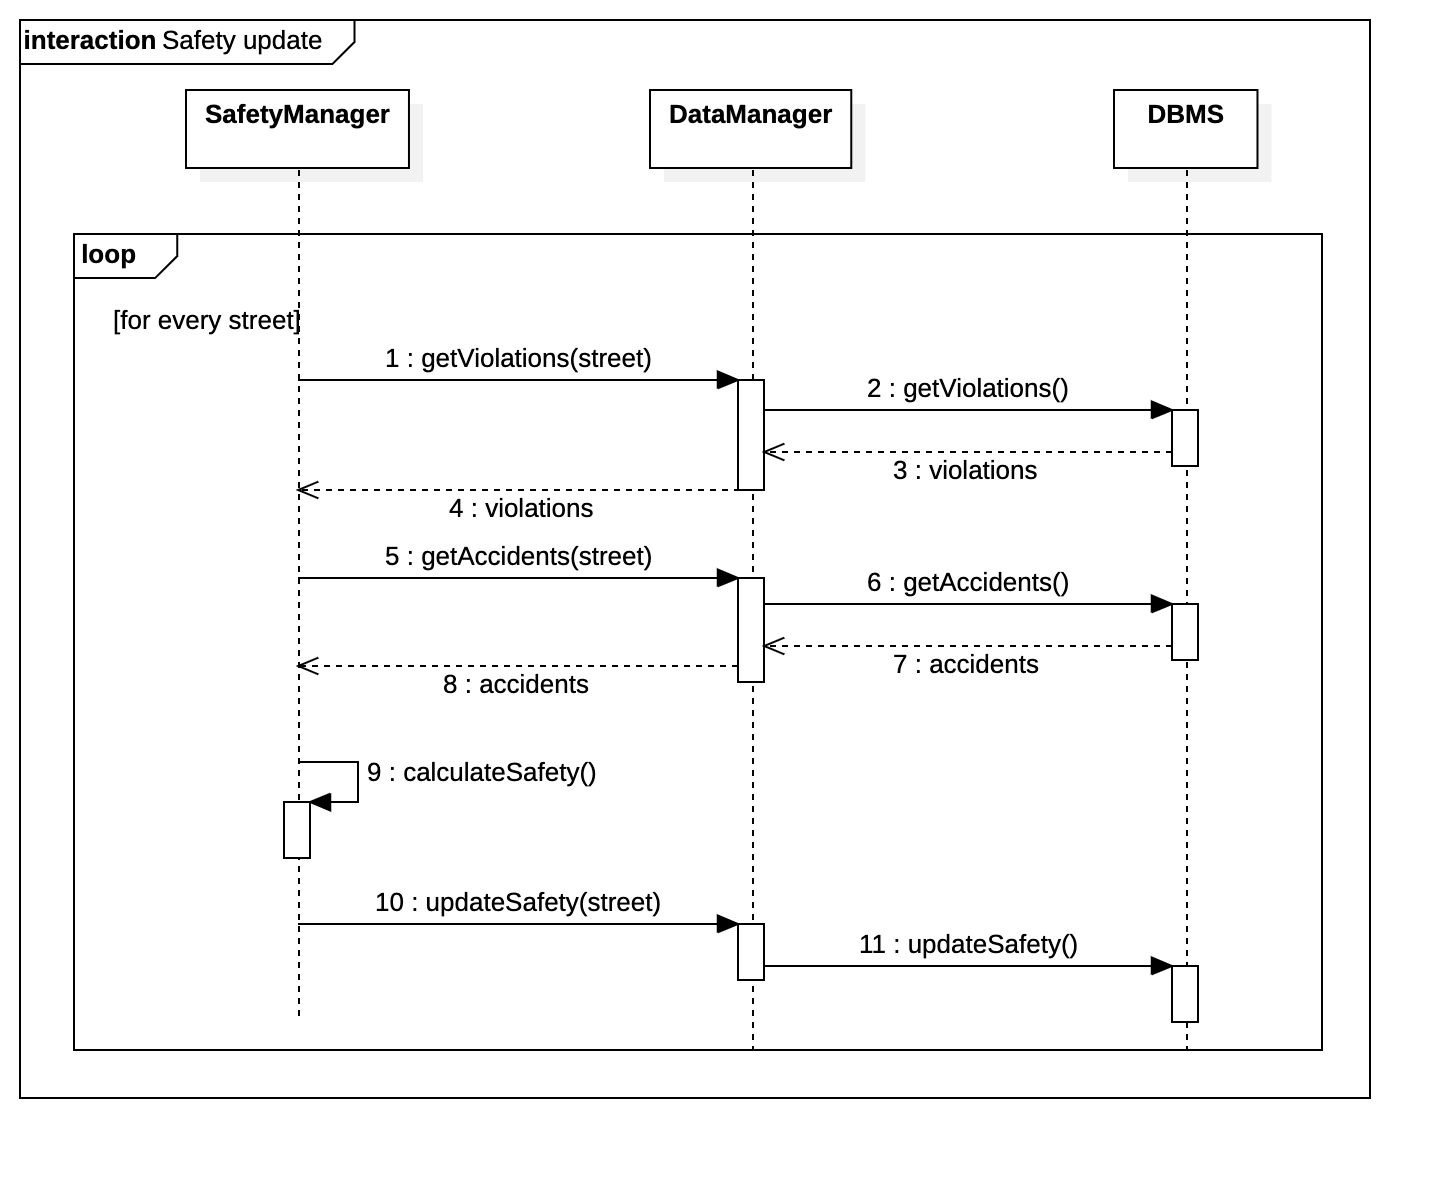
\includegraphics[scale=0.14]{dd/safetyUpdate}
			\end{figure}
		\end{frame}
	
	\subsection{Architectural Styles and Patterns}
		\begin{frame}{Client-Server in Four-tier Architecture}
			The system is a \textbf{crowed-sourced} application based on the client-server paradigm where the \emph{users} represent the crowd on which the functionalities of SafeStreets are funded.
			
			\begin{figure}[h!]
				\centering
				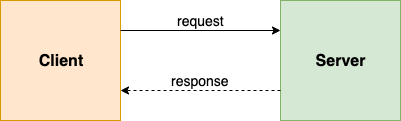
\includegraphics[scale=0.32]{dd/clientServer}
			\end{figure}
		
			The layers of the system are deployed to a \emph{four-tier architecture}.
			
			\begin{figure}[h]
				\centering
				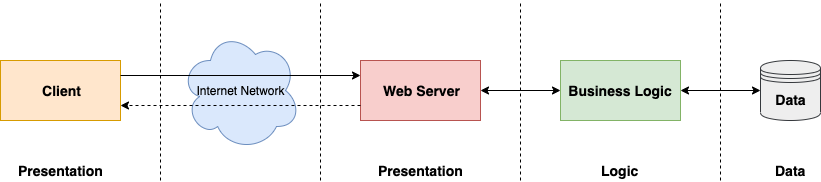
\includegraphics[scale=0.32]{dd/fourTierArchitecture}
			\end{figure}
		\end{frame}
	
		\begin{frame}{REST and TCP/IP}
			SafeStreets provides its services through \textbf{REST} thanks to an interface that is extended twice to define the communication with the \textbf{mobile app} for the users and the \textbf{web app} for the authorities.
			
			\begin{figure}
				\begin{minipage}{0.42\textwidth}
					\centering
					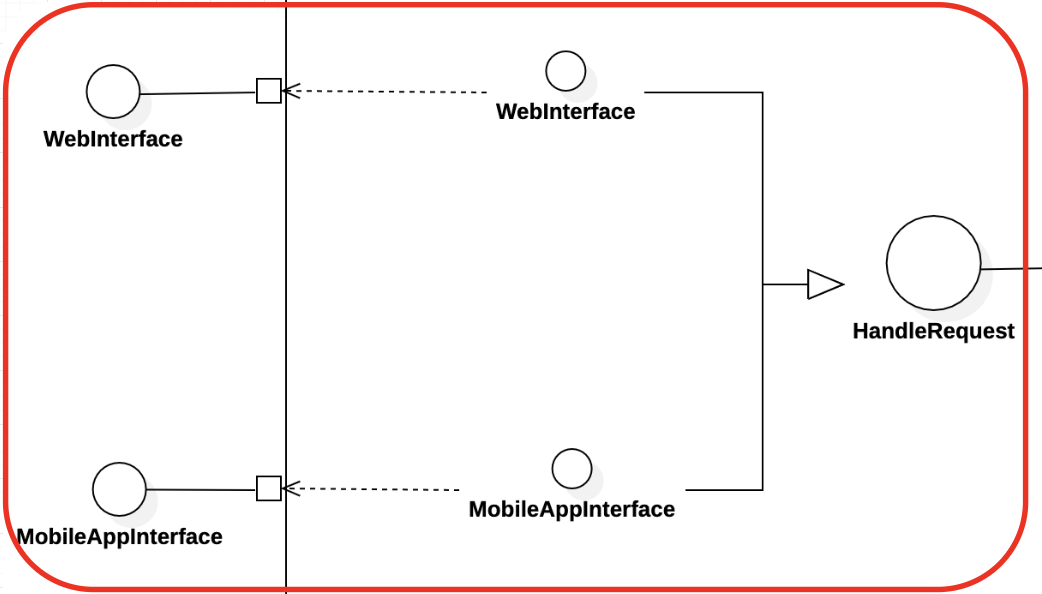
\includegraphics[scale=0.25]{dd/restInterface}
				\end{minipage}
				\begin{minipage}{0.3\textwidth}\tiny
					\color{polimiblue}Client-Handler Component Interfaces Particular
				\end{minipage}
			\end{figure}
			
			Moreover basic communication with the TCP/IP protocol is also used in particular for the external components that allows the system to manage its data: the \emph{DBMS} and the \emph{EMS}.
		\end{frame}
		
	\subsection{Deployment View}
		\begin{frame}{Deployment View}
			\begin{figure}[hbtp]
				\vspace{-10pt}
				\centering
				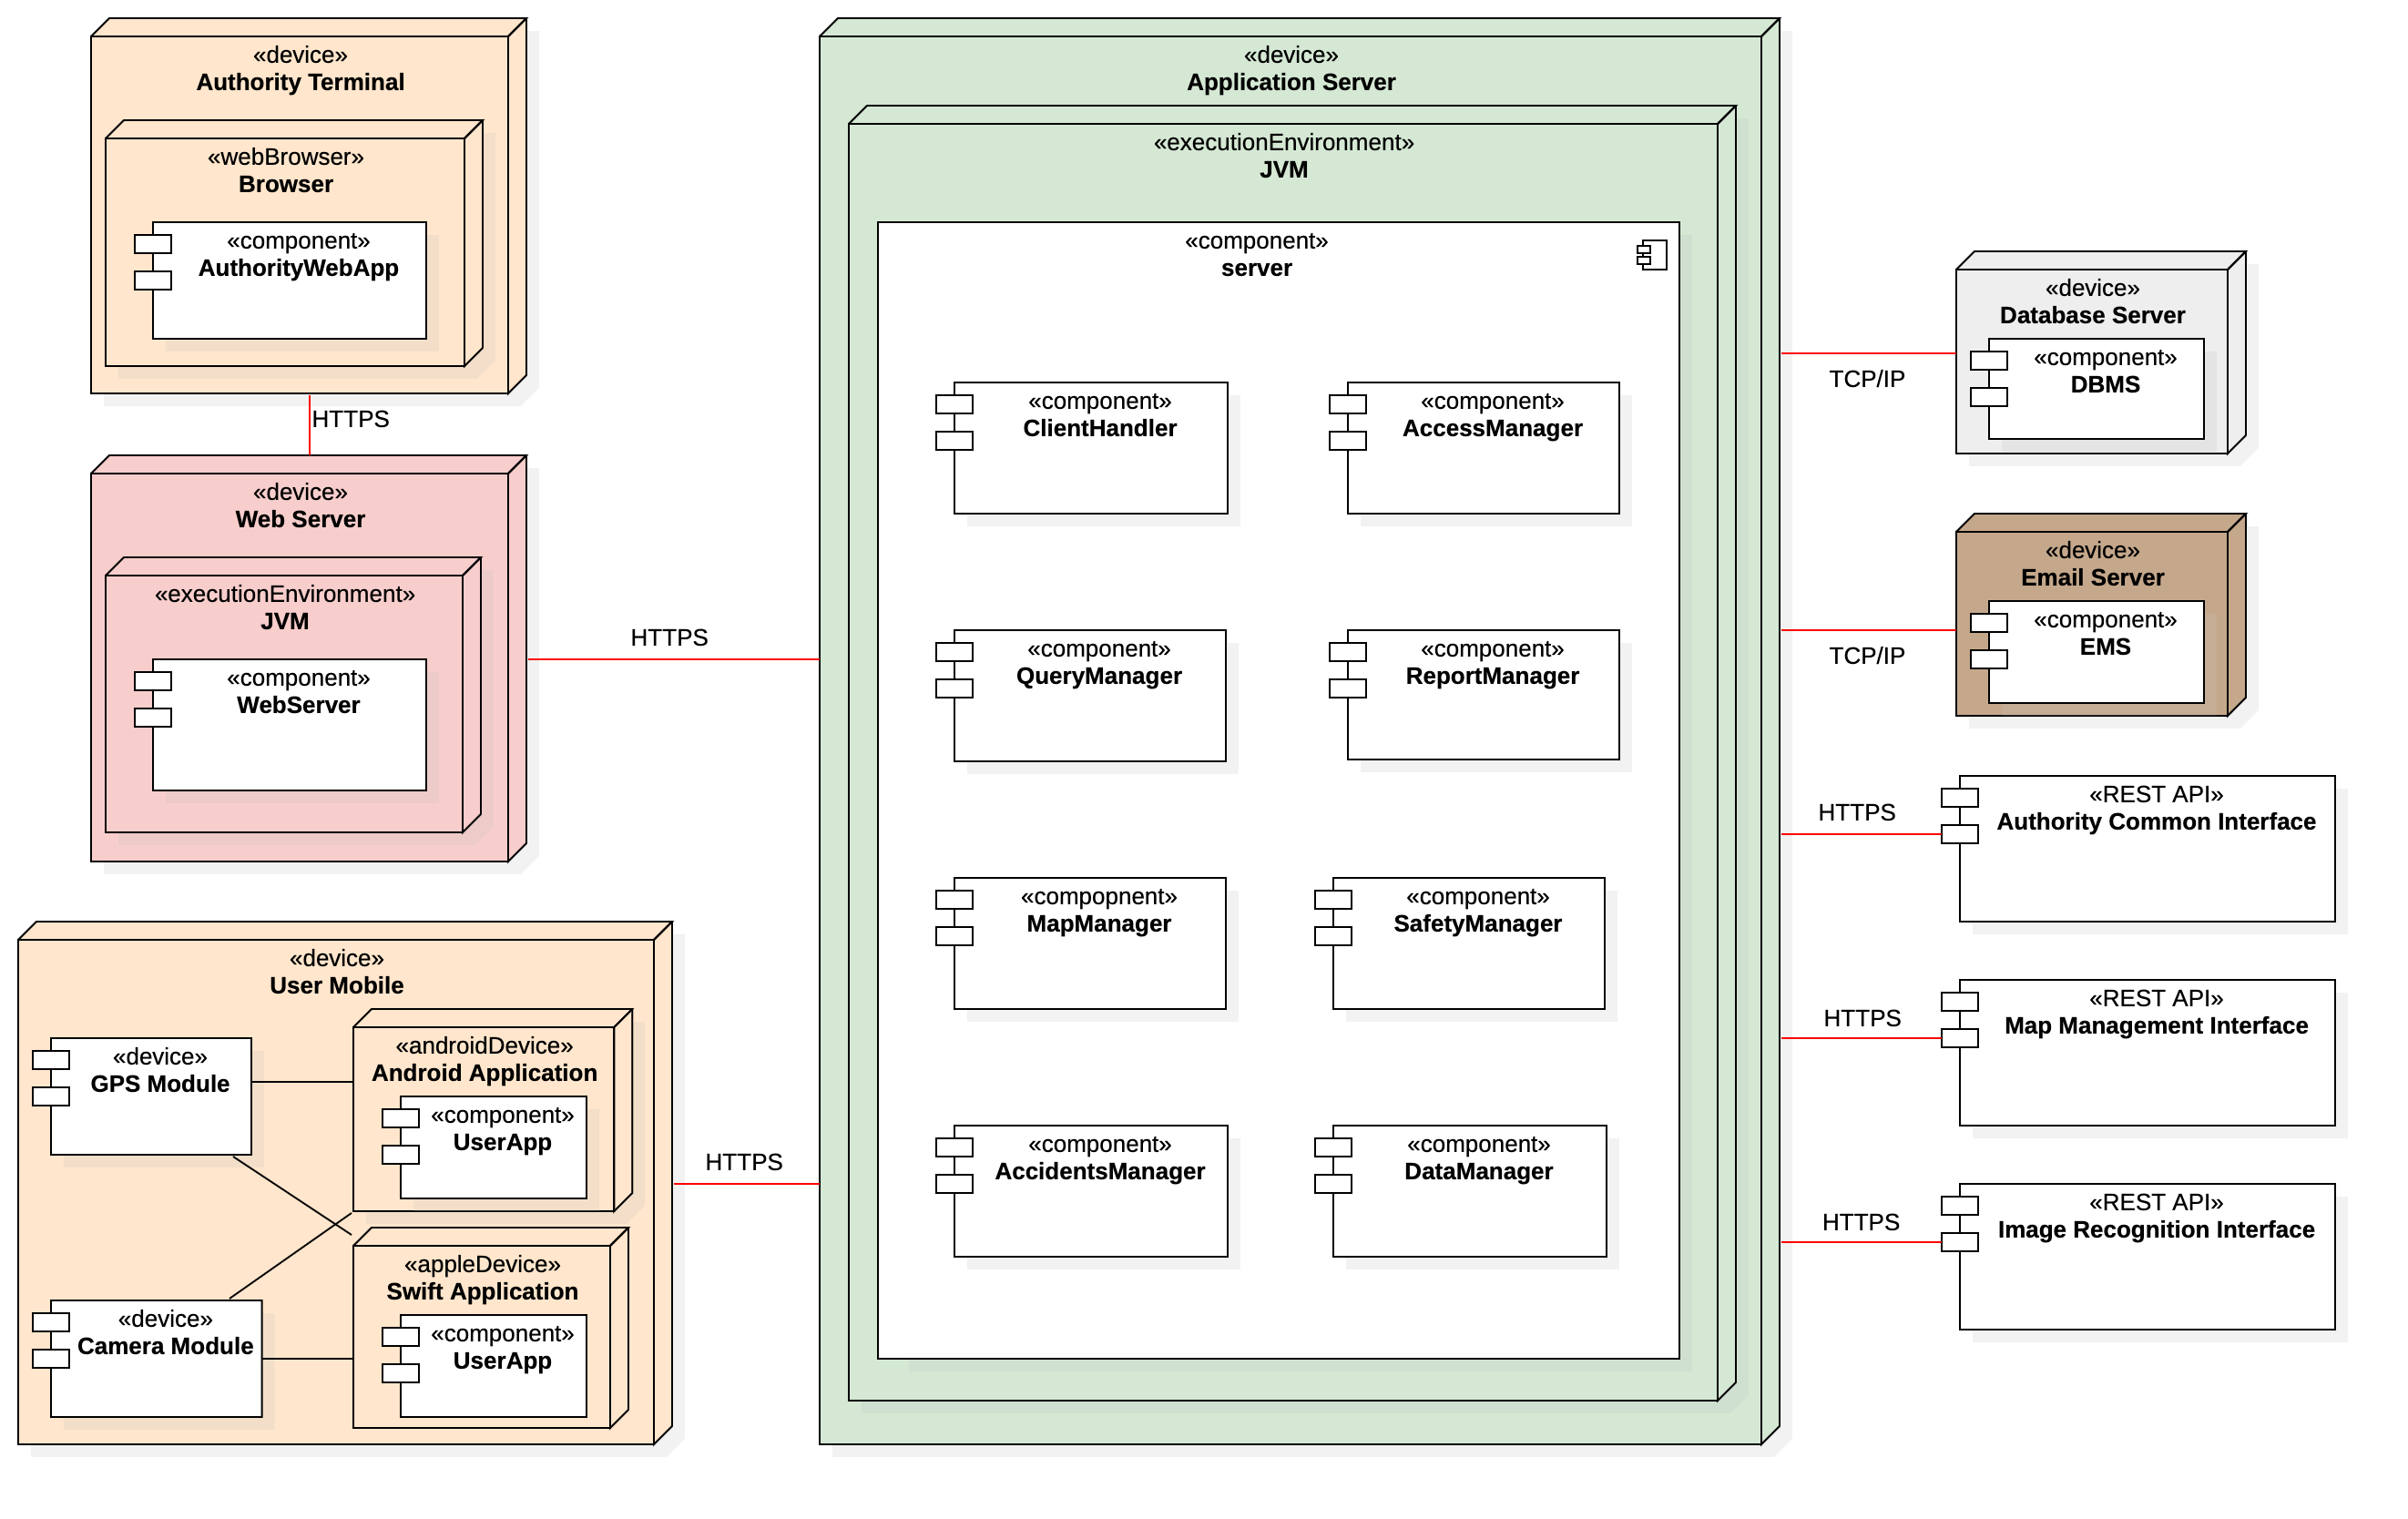
\includegraphics[scale=0.12]{dd/deploymentDiagram}
			\end{figure}
		\end{frame}
	
	\subsection{Implementation Integration and Test Plan}
		\begin{frame}{Strategy Overview}
			\vspace{-2cm}
			The strategy on which the \emph{Implementation, Integration and Test Plan} is developed, and thus the use relation hierarchy diagram, is based on the following 4 features:
			
			\vspace{1cm}
			\begin{itemize}
				\item[1.] <1-> \textbf{Bottom-Up and Top-Down approach}
				\item[2.] <2-> \textbf{Core Functionality}
				\item[3.] <3-> \textbf{Decoupling of Components}
				\item[4.] <4-> \textbf{Reliability of Eternal Systems}
			\end{itemize}
		\end{frame}
	
		\begin{frame}{Use Relation Hierarchy Diagram}
			\begin{figure}
				\vspace{-10pt}
				\centering
				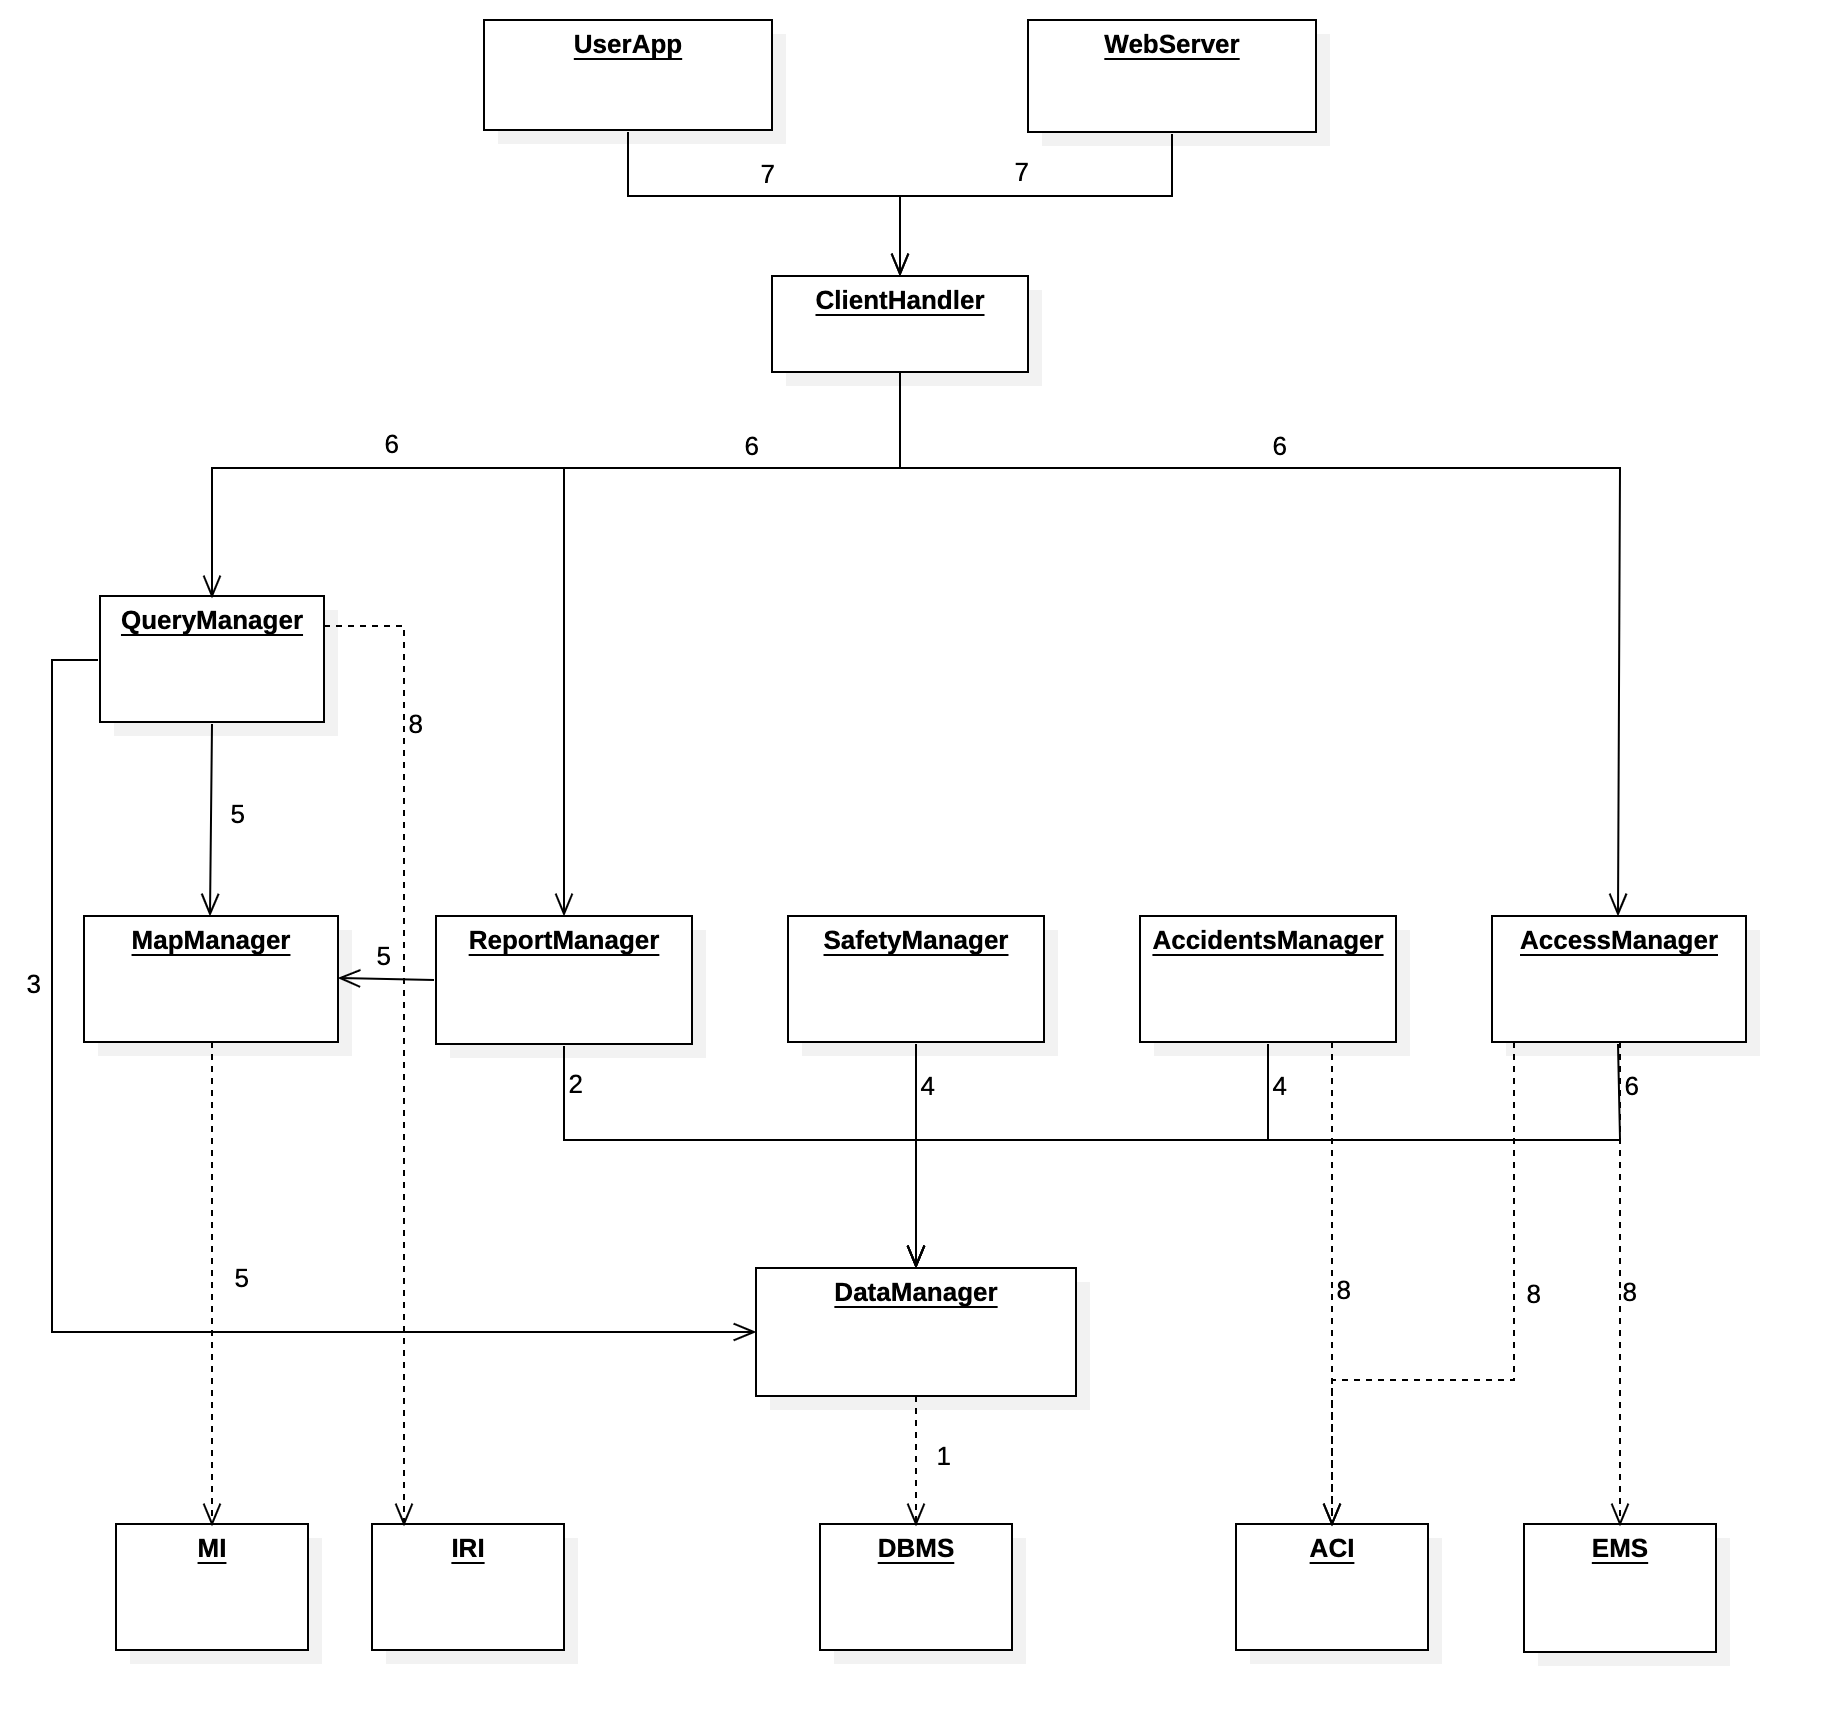
\includegraphics[scale=0.13]{dd/useRelationHierarchy}
			\end{figure}
		\end{frame}